%% Electro-optic study of AlGaAs coated mirrors

 As mentioned in Section (1?) one of the many LIGO fundamental noise sources is coating thermal noise from the $\mathrm{SiO_2}/\mathrm{TiO_2:Ta_2O_5}$ aLIGO coatings. As aLIGO approaches its designed sensitivity various coating solutions are currently proposed to mitigate thermal noise coupling into the detector output.
With the potential to reduce coating Brownian noise by a factor of 10 \cite{Cole:2013}, $\mathrm{Al_{.92}Ga_{.08}As}$ shows much promise with next generation detector with a corresponding strain reduction by a factor of (5?) in comparison to the aLIGO coatings, though with different material properties of these crystalline coatings introduce new coating noise couplings.

A notable source of noise is the linear electro-optic property of the crystalline material (dn/dE), also known as the Pockels effect \cite{abernathy_poster}. Characterizing currently proposed $\mathrm{Al_{.92}Ga_{.08}As}$ coated "witness" samples thorough extensive analysis and experimental data of the aforementioned property is essential for the use of $\mathrm{Al_{.92}Ga_{.08}As}$ coatings in gravitational wave interferometers. The following section dedicated to the discussion of the linear electro-optic effect starting with the fundamentals on anisoptropic media and the electro-optic tensor of zincblende crystalline materials, estimates of the differential phase of light reflected from a GaAs/$\mathrm{Al}_{0.92}\mathrm{Ga}_{0.08}\mathrm{As}$ coating, and an experiment constructed with the intention of measuring the linear electro-optic effect within a 1kHz $\rightarrow$ 1MHz region.

\subsection{Thermal noise}
 In 1827, the Scottish botanist Robert Brown noticed a constant motion of pollen particulates on the surface of water; which we now know was due to the randomized collisions of the water molecules holding a kinetic energy proportional to the temperature ($k_BT$) \cite{Brown:1828}. It is because of his documented observations we name the phenomena Brownian motion. Further insight into Brownian motion was explored by Einstein where he was able to relate the mean-square displacement of a particle of radius $r_\mathrm{sph}$ on a fluid with viscosity $\eta$.

 \begin{equation}
 \overline{x^2} = k_B T  \frac{1}{3 \pi \eta  r_\mathrm{sph}}
 \end{equation}

 This relation has important implications about how the random motion or fluctuations of a particulate (the pollen) is influenced (dissipated) by the viscosity of the surrounding medium (water). In fact, Brownian motion belongs to a unique set of statistical thermodynamic systems that obey the Fluctuation-Dissipation theorem. Derived by H.B. Callen and T.A. Welton, the theorem states that for a randomly fluctuating linear force \cite{Callen:1951}:

\begin{equation}
F_x^2(f) = 4 k_B T\; \Re[\eta]
\end{equation}

 \noindent Where $\Re[\eta]$ is the real part of the viscosity or more generally the impedance of the system. This impedance directly relates to equations of motion:

 \begin{equation}
 \eta = \frac{F}{\dot{x}}
 \end{equation}

\noindent Another useful form is the power spectrum of the fluctuating motion:
\begin{equation}\label{fdtpsd}
x^2 (f)  = \frac{4k_B T}{(2 \pi f)^2}\; \Re[Y]
\end{equation}

Where $Y$ is the inverse of the impedance or admittance. With this power spectra, modelling and budgeting notable LIGO fundamental noise contributions attributed to the choice of the materials used for highly reflective mirror coatings, mirror and lens substrates, and pendulum fibers used to suspend core optics becomes significantly less daunting. Though the next step requires adequate modelling of internal force couplings for the aforementioned components.
\\
\textbf{Internal friction in Materials and Loss angle}
\\
Zener provides a model of the internal friction of materials incorporating anelasticity into the equations of motion \cite{zener:1948}:

\begin{equation}
F = k(1+i\phi)x + m\ddot{x}
\end{equation}

Where $m$ is mass attached to a spring with a spring constant $k(1+ i\phi)$ incorporating the degree of anelasticity $\phi$. From equations 3.5 and 3.3 we perform a Laplace transform and acquire the following form of admittance:
\begin{equation}
Y(s) = \frac{\dot{x}(s)}{F(s)} = \frac{-s}{k(1+i\phi) + ms^2}
\end{equation}

\noindent Or more transparently the Fourier representation since we assume a linear time invariant system:

\begin{equation}\label{admitint}
Y(\omega) = \frac{\dot{x}(\omega)}{F(\omega)} = \frac{-i\omega}{k(1+i\phi) - m\omega^2} = \frac{k \omega \phi - i \omega (k - m \omega^2)}{(k-m\omega^2)^2 +k^2 \phi^2}
\end{equation}

\noindent Plugging equation \ref{admitint} back into \ref{fdtpsd}:

\begin{equation}
x^2 (f)  = \frac{2k_B T}{\pi}\frac{k\phi}{(k-4\pi^2 m f^2)^2 + k^2 \phi^2}
\end{equation}

\noindent Still, computing the admittance from a Gaussian beam impinging upon a HR mirror is not at all trivial and can require one to expand all individual mechanical modes of oscillation of the test mass system across a relevant frequency range. Saulson and Gonzalez provide an alternative method to computing the admittance coined the ``direct approach" by Levin when computing the noise from a Gaussian beam on a LIGO HR test mass \cite{levin:1998}. The admittance can be acquired through:

\begin{equation}
\Re[Y] = \frac{W_\mathrm{diss}}{F_o^2}
\end{equation}

\noindent $W_\mathrm{diss}$ is the dissipated power from the system due to an oscillating force $F_o$. In the case of the beam/optic system studied by Levin, this requires that the driving force used in a lab mimics that of a force from a centered Gaussian beam.
\\
\\
\noindent \textbf{Coating thermal noise}
\\
Further investigations into the beam/optic system utilizing this approach and elasticity theory led to a deeper understanding about brownian thermal noise contributions from LIGO test masses (substrate, suspensions, HR coating). Levin mentions, with details from Harry that the noise contributed by a lossy mirror coating can prove to be the most significant contributor of brownian thermal noise. Hong provides a power spectral density \cite{Hong:2013}:

\begin{equation}
S_j^X = \frac{4k_B T \lambda \phi_x^j(1- \sigma_j - 2 \sigma_j^2)}{3 \pi^2 f Y_j (1-\sigma_j)^2 \omega_o^2}
\end{equation}

X = Bulk and Shear
with alternating layers j = odd (material 1) j = even (material 2)
\\
\textbf{current $\mathrm{SiO_2}/\mathrm{TiO_2:Ta_2O_5}$ elasticity params, power spectra, and strain spectral density (order of magnitude estimate)} \cite{Harry:06}
\\
\noindent \textbf{Benefits of AlGaAs (elasticity params, power spectra, strain spectral density (order of magnitude estimate)} \cite{Cole:2013}

\noindent Currently thermal noise from the $\mathrm{SiO_2}/\mathrm{TiO_2:Ta_2O_5}$ optical coatings is the largest contributor of Brownian noise in LIGO compared to estimated substrate and suspension thermal noise \cite{Harry:06}. As of the end of O3, Brownian thermal noise is estimated to be ? orders of magnitude below the current sensitivity and it will prove to be the limiting source of noise as that sensitivity is increased with various other upgrades mitigating fundamental and technical noise. (\textcolor{red}{already mentioned in intro prior to this thermal noise section. Need to re-iterate in more detail?})
 \\
 \\


\subsection{Anisotropic media and birefringence}
Unlike with isotropic media, we cannot assume that the index of refraction of anisotropic media is the same for all chosen wave vectors. This is a direct consequence of the birefringence of anisotropic media; characterized by the dielectric, permittivity, and polrization tensors. The relation between the displacement vector and electric field:

\begin{equation}
D_i = \varepsilon_{ij}E_j
\end{equation}
Where i=j for isotropic media.
\\
\\
\textcolor{red}{Yariv (Chapter 5)}
\\
Uses the Poynting theorem to show the case where assuming the same energy flux through isotropic and anisotropic media leads to principle dielectric axes for the latter.
\\
\textcolor{red}{Go through some brief math to show how the property of birefringence deduces the nature of a indicatrix and ordinary and extraordinary axes. }\cite{yariv, nye}
\\
\\
\textcolor{red}{Nye (Chapter 8.2)}
\\
\\
\textcolor{red}{Born and Wolf (Chapter 15)}
\\
\subsubsection{The electro-optic tensor and the Pockels effect}
Some anisotropic crystalline media (ACM) exhibit characteristics where the indicatrix changes as a function of a slowly (\satoshi{is this statement correct?}) (\textcolor{red}{up to the speed of sound within the media?}) varying electric field ~\cite{yariv,nye}.
\\
\textcolor{red}{Indicatrix with electro-optic coefficients.}
\\
Relationship between a slowly varying electric field vector of an arbitrary direction $\vec{E} = [E_1, E_2, E_3]$ to the perturbations of the indicatrix:
\\
\begin{equation}
  \left[ {\begin{array}{c}
   \big( \frac{1}{\Delta n ^2 } \big)_1 \\
   \big( \frac{1}{\Delta n ^2 } \big)_2 \\
   \big( \frac{1}{\Delta n ^2 } \big)_3 \\
   \big( \frac{1}{\Delta n ^2 } \big)_4 \\
   \big( \frac{1}{\Delta n ^2 } \big)_5 \\
   \big( \frac{1}{\Delta n ^2 } \big)_6 \\

  \end{array} } \right]
  =
%
 \left[ {\begin{array}{ccc}
   r_{11} & r_{12} & r_{13}\\
   r_{21} & r_{22} & r_{23}\\
   r_{31} & r_{32} & r_{33}\\
   r_{41} & r_{42} & r_{43}\\
   r_{51} & r_{52} & r_{53}\\
   r_{61} & r_{62} & r_{63}\\
  \end{array}} \right]
 %
 \left[{\begin{array}{c}
   E_1\\
   E_2\\
   E_3\\
 \end{array}} \right]
\end{equation}

The six indices correspond to the six unique elements in the indicatrix.
\\
\\
\textcolor{red}{Nye (Chapter 8.2)}
\\
\\
\textcolor{red}{Yariv (Chapter 14)}
\\
\\
\textcolor{red}{ How the modulation of the phase of the carrier field is dependent on the orientation of its wave vector with respect to the crystal structure, the modulating electric field direction and strength, (other items to discuss in terms of introducing the effect)}
\\
This property of ACM is what allows electro-optic modulators to operate as light phase modulators

\subsubsection{Electro-optic tensor for zincblende structures with $\bar{4}3m$ point group symmetry}
\begin{equation}
 \left[ {\begin{array}{ccc}
   0 & 0 & 0\\
   0 & 0 & 0\\
   0 & 0 & 0\\
   r_{41} & 0 & 0\\
   0 & r_{41} & 0\\
   0 & 0 & r_{41}\\
  \end{array} } \right]
\end{equation}
\\
$r_{41} = r_{52} = r_{63}$
\\
For GaAs @ $10.6\mu$ $r_{41} = 1.6 \times 10^{-12}$ [m/V]
\\
Adachi estimate for $\mathrm{Al_{x}Ga_{1-x}As}$?



\section{Phase modulation of light propogating through a anisotropic crystalline thin film stack}

\subsection{Coating parameters}

\textcolor{red}{Is the sample that we have a standard AlGaAs sample from Thorlabs/CMS?}


\subsubsection{Growth orientation (Miller indices) with respect to substrate surface}
\begin{itemize}
\item Mirror surface is the [100] plane.
\item Within the [100] plane the AlGaAs coating is grown with a flat indicator that draws a line within the [0-11] plane where the surface normal is pointing towards the sample center.
\end{itemize}


\subsubsection{Layering}
The coating to be studied consists 36 $\lambda$ / 4 (\satoshi{remove unnecessary space $\lambda/4$}) thick layers of GaAs interspersed with 35 layers of $\lambda$ / 4 thick AlGaAs.   GaAs forms the top and bottom layer to protect the AlGaAs from absorbing oxygen from the air.
High Index:  GaAs, n=3.480, layer thickness is 76.43 nm
Low Index:  $ \mathrm{Al}_{0.92} \mathrm{Ga}_{0.08} \mathrm{As} $, n=2.977, layer thickness is 89.35 nm
\textcolor{red}{Info from Steve. Written source?}


\subsection{Fejer and Bonilla estimate (analytical approximation)}
Fejer and Bonilla take an analytical approximation approach when finding the impact of the electric field to the change in phase of the light through a crystalline anisotropic thin film ($\lambda/4$) stack \cite{bonilla_fejer}.

\begin{equation}
\hat{\phi}' = \frac{\pi n_1 z}{1-z^2}(z^{2N} -1) \frac{z^{2N} \frac{(n_f)^2}{n_2 n_3}(n_2 \kappa_{\gamma 2} + n_3\kappa_{\gamma 3}) - (n_2 \kappa_{\gamma 3} + n_3\kappa_{\gamma 3})}{(n_1)^2 -(n_f)^2 z^{4N}}
\end{equation}

with $z = \frac{n_2}{n_3}$
and
$
\kappa_{\gamma j} = \frac{d}{d \gamma} \mathrm{log}(n_j h_j)|_{\gamma =\gamma_{O}} \bigg(\frac{\hat{n}_j'}{\hat{n}_j} +\frac{\hat{h}_j'}{\hat{h}_j} \bigg)
$

With $\kappa$ being a scalar parameter.

\satoshi{Adding a schematic would be helpful.}

\subsection{Ballmer estimate (numerical)}

In the appendix of \cite{ballmer2015} Ballmer explains a formalism that allows the coating transfer function given a differential change in phase due to a scalar parameter to be expressed as follows:

\begin{equation}
M = Q_N D_N ...Q_kD_k...Q_1D_1Q_0
\end{equation}

For a single pass through the coating where the coating thickness and indices are left general.

\satoshi{Both approaches are essentially based on the same calculation method i.e., transfer matrices.}

\section{Projected DARM coupling}
To estimate how much DARM coupling can occur, we use use a measured field spectra acquired from installed electric field meters located within LIGO Hanford Observatory EX and EY vacuum chambers. Taking the upper and the lower EFM measurements in $.3\; [\mathrm{V}/\mathrm{m}/\sqrt{\mathrm{Hz}]}$ @ 60 Hz and $4\times10^{-3}\; [\mathrm{V}/\mathrm{m}/\sqrt{\mathrm{Hz}]}$ @ 4kHz ~\cite{efm_log}.
\satoshi{I don't think these values are calibrated. According to Martynov et al. 2016, the fluctuations in the electric filed is $\sim10^{-5}\,\mathrm{[(V/m)/\sqrt{Hz}]}$.}
This along with computed estimate above allows us to create an upper limit for what this noise might be assuming incoherent fields between the end stations and a flat frequency response within LIGO's bandwidth.

\section{Experiment}
To probe for this effect, we took the approach of an in-air Fabry-P\'{e}rot cavity with a GaAs/$\mathrm{Al_{.92}Ga_{.08}As}$ coated sample end mirror mounted in a custom designed MACOR mount with the ability to install electrodes maintaining a fixed distance from the sample surfaces for a controlled E-field injection. Details and specifications are discussed as well as relevant measurements. An improved experimental design is also detailed for a higher sensitivity measurement.

\subsection{Design}
This section details the Pound-Drever-Hall servo which is at the heart of this experiment, the on-table design, a sample / electrode assembly used for a controlled electric field injection, and electrode drive parameters
\subsubsection{PDH servo}
The Pound-Drever-Hall technique, originally imagined for laser frequency stabilization to an ultra-stable length reference, achieves constant resonance with said reference by tracking the phase of the cavity input light with respect to the light reflected from the cavity. Tracking the approximately linear phase response across resonance is at the heart of this technique and recognizes that physical property to be probed around a cavity's resonance cannot be the intensity of the transmitted or reflected light because of the quadratic symmetry. (\textcolor{red}{Derivative of the intensity could work but depends on us operating off resonance})
\\
\textcolor{red}{Insert figure of reflected intensity and phase response around resonance (cavity transfer function). Maybe also have a figure corresponding to what this could represent in a lab. (sweeping a mirror of the laser cavity through resonance)}
\\
Another novelty and insight to the technique is the use of phase modulation onto the carrier field which is the mathematical and physical equivalent to imposing separate optical fields which in most cases do not resonate in the optical cavity.
\\
\begin{equation}
E_\mathrm{inp} = E_o e^{i \omega t + \beta \mathrm{sin}( \Omega t)}
\end{equation}

\textcolor{red}{Approximation with Bessel functions (assumptions about modulation depth)}
\begin{equation}
E_\mathrm{inp} \approx E_o \satoshi{E_0} [J_o\satoshi{J_0}(\beta)e^{i \omega t} + J_1(\beta)e^{i (\omega + \Omega) t} - J_1(\beta)e^{i(\omega -\Omega)t}]
\end{equation}
\\
\textcolor{red}{Discuss how the measurement of the beat power between the sideband and the carrier at the RFPD tracks the phase and how with demodulation and filtering, you can create an error signal.}

\begin{figure}[H]
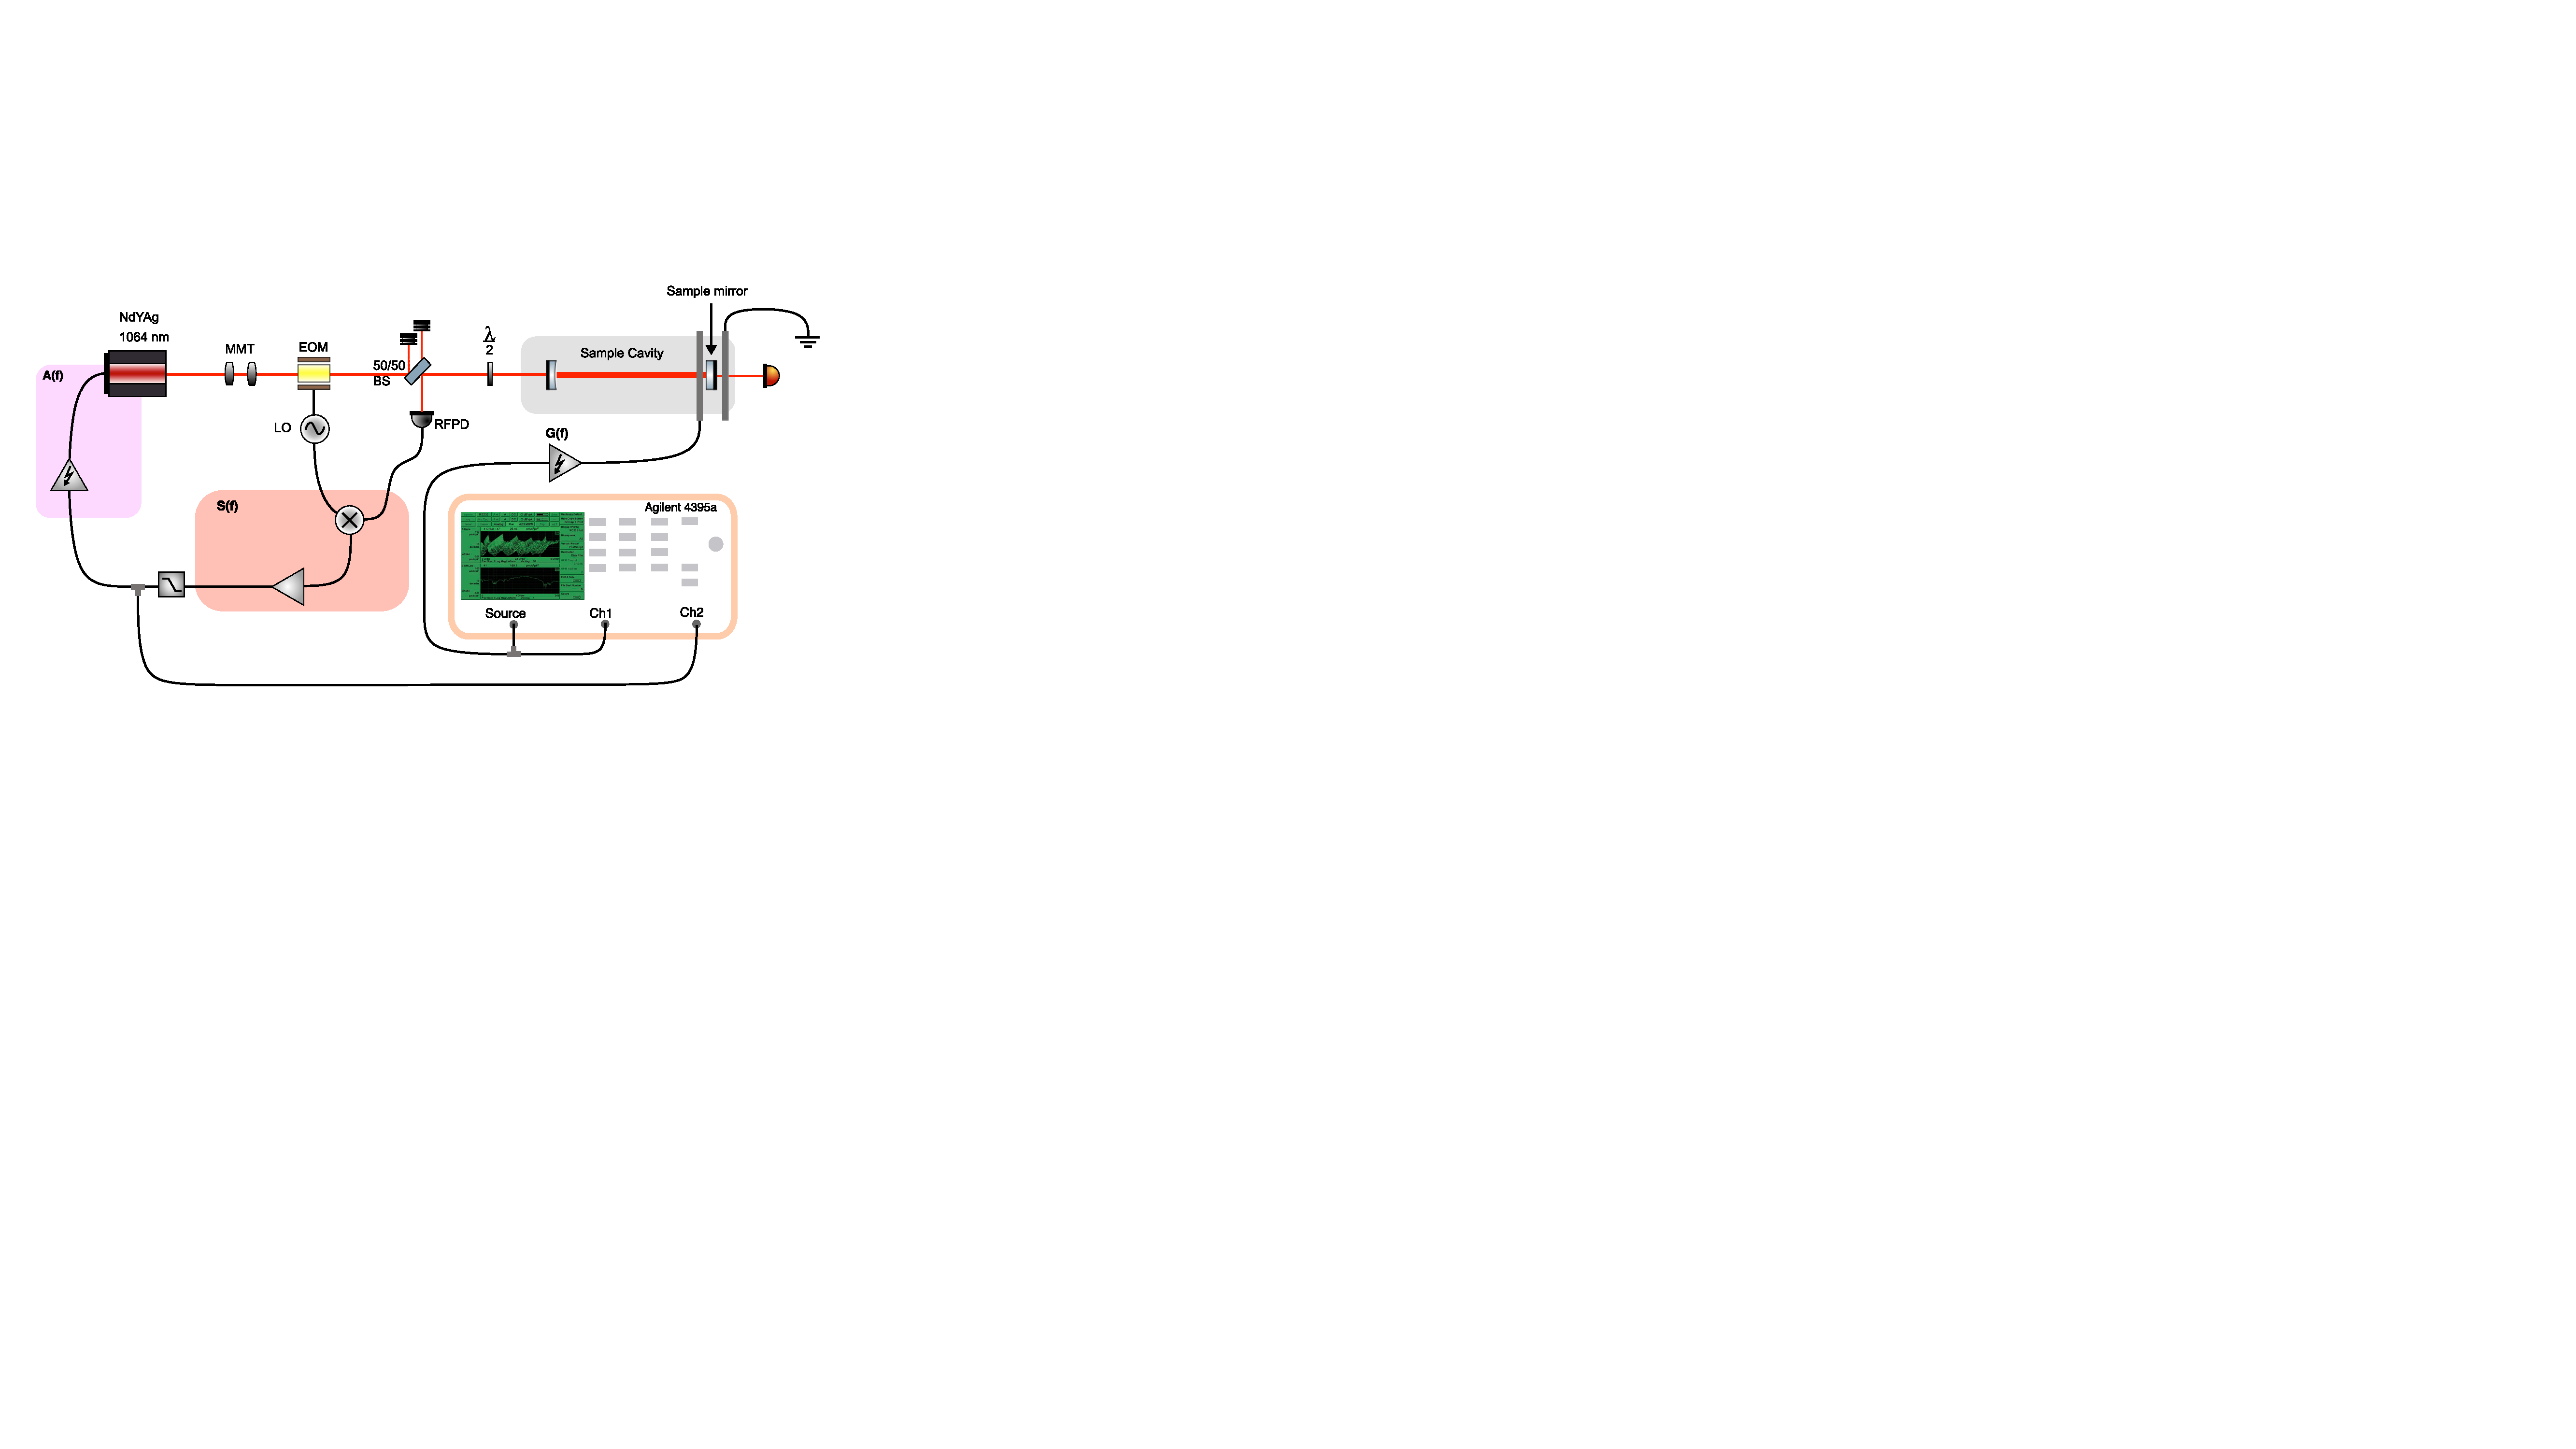
\includegraphics[width=\textwidth]{figs/ALGAAS/electrooptic_study_algaas_0.pdf}
\caption{Simplified experiment schematic}
\label{fig:poisson_output}
\end{figure}

\subsubsection{On-table schema}

\textcolor{red}{A figure that highlights path that is intended for locking onto the PMC, and a different color highlight for the path to the experiment}

The setup presented in this section, branches off of a previously established optical path used to lock onto a separate optical cavity (PMC).
\\
The laser light source is a Mephisto 2000 NE 1064nm laser.
\\
25 MHz EOM is a New Focus Model 4003 IR resonant phase modulator.
\\
The designed cavity is a .1651 m \satoshi{$0.1651\,\mathrm{m}$ ($0$ should not be ommited in scientific articles)} long cavity with a HR IBS coated sample (PL-CC, ROC =.333 m) input coupler from CVI Melles-Griot and a GaAs/$\mathrm{Al_{.92}Ga_{.08}As}$ (PL-PL) fused silica substrate by the Crystalline Mirror Solutions (CMS) division of Thorlabs with the aforementioned parameters (\textcolor{red}{mentioned in coating parameters section}).

\subsubsection{Sensing S(f)}
\begin{itemize}
\item 25 MHz RFPD
\begin{itemize}
\item Transimpedance measurement (necessary? or should I just use the mixer out PDH to summarize PD/mixer response)
\end{itemize}
\item Frequency Stabilization servo (modified MIT FSS (DCCD980536)) (LTspice model in appendix)
\end{itemize}


\subsubsection{Actuation A(f)}
\begin{itemize}
\item Mephisto 2220 PZT response (capacitance estimated from HVA drive measurement with and without connection to PZT)
\item Channel 3 of SVR 350-3 BIP High Voltage Amplifier from Piezomechanik GmbH with Pomona box (elog 412)
\item \textcolor{red}{Figure of frequency response of A(f)}

\end{itemize}

\subsubsection{Low frequency servo (Thermal loop)}
\begin{itemize}
\item Passed signal from FSS $\rightarrow$ integrators $\rightarrow$ Laser thermal actuator input
\end{itemize}

\subsubsection{OLG(f)}
Isn't quite $\mathrm{A}(f)*\mathrm{S}(f)$ as stated. Doesn't entirely account for the optical plant.
How the measurement is taken (important to take between installations to account for the changes in the optical plant) (elog 831)


\subsubsection{Sample / Electrode assembly}
Maximizing the electric field ($|E_z|$) and within the coating while requiring a through beam to and through the HR coating lead us to imagine disk electrodes with a 3mm central aperture. The aperture size was chosen to be at least 5 times larger than the beam size at the plate locations. This was to avoid any beam clipping while still allowing to maximize the field strength at the region of interest.
\\
Most commercial optical mounts are conductive which proved to be a problem when attempting to find a mounting solution while reducing the non-normal field gradients within the volume of interest around the sample. Because of this, we chose to construct an optical mount made of MACOR a machinable ceramic with high a high Young's modulus (66.9 GPa), and a moderate Poisson ratio (.29) \cite{macor}. An optical mount for the sample made with MACOR, along with glass bearnings .48 $\pm$ .01 cm $\diameter$  and a McMaster-Carr 8-32, 1/2" ceramic screw were used to clamp and suspend the optical sample. A 1.24" $\diameter$ hole was bored into the MACOR with a (\textcolor{red}{depth?}) depth so that there is a ? mm clearance between the front and back surface of the sample to the electrode plates.
\textcolor{red}{Figure with  the sample in-situ}
\\
\begin{figure}[H]
\centering
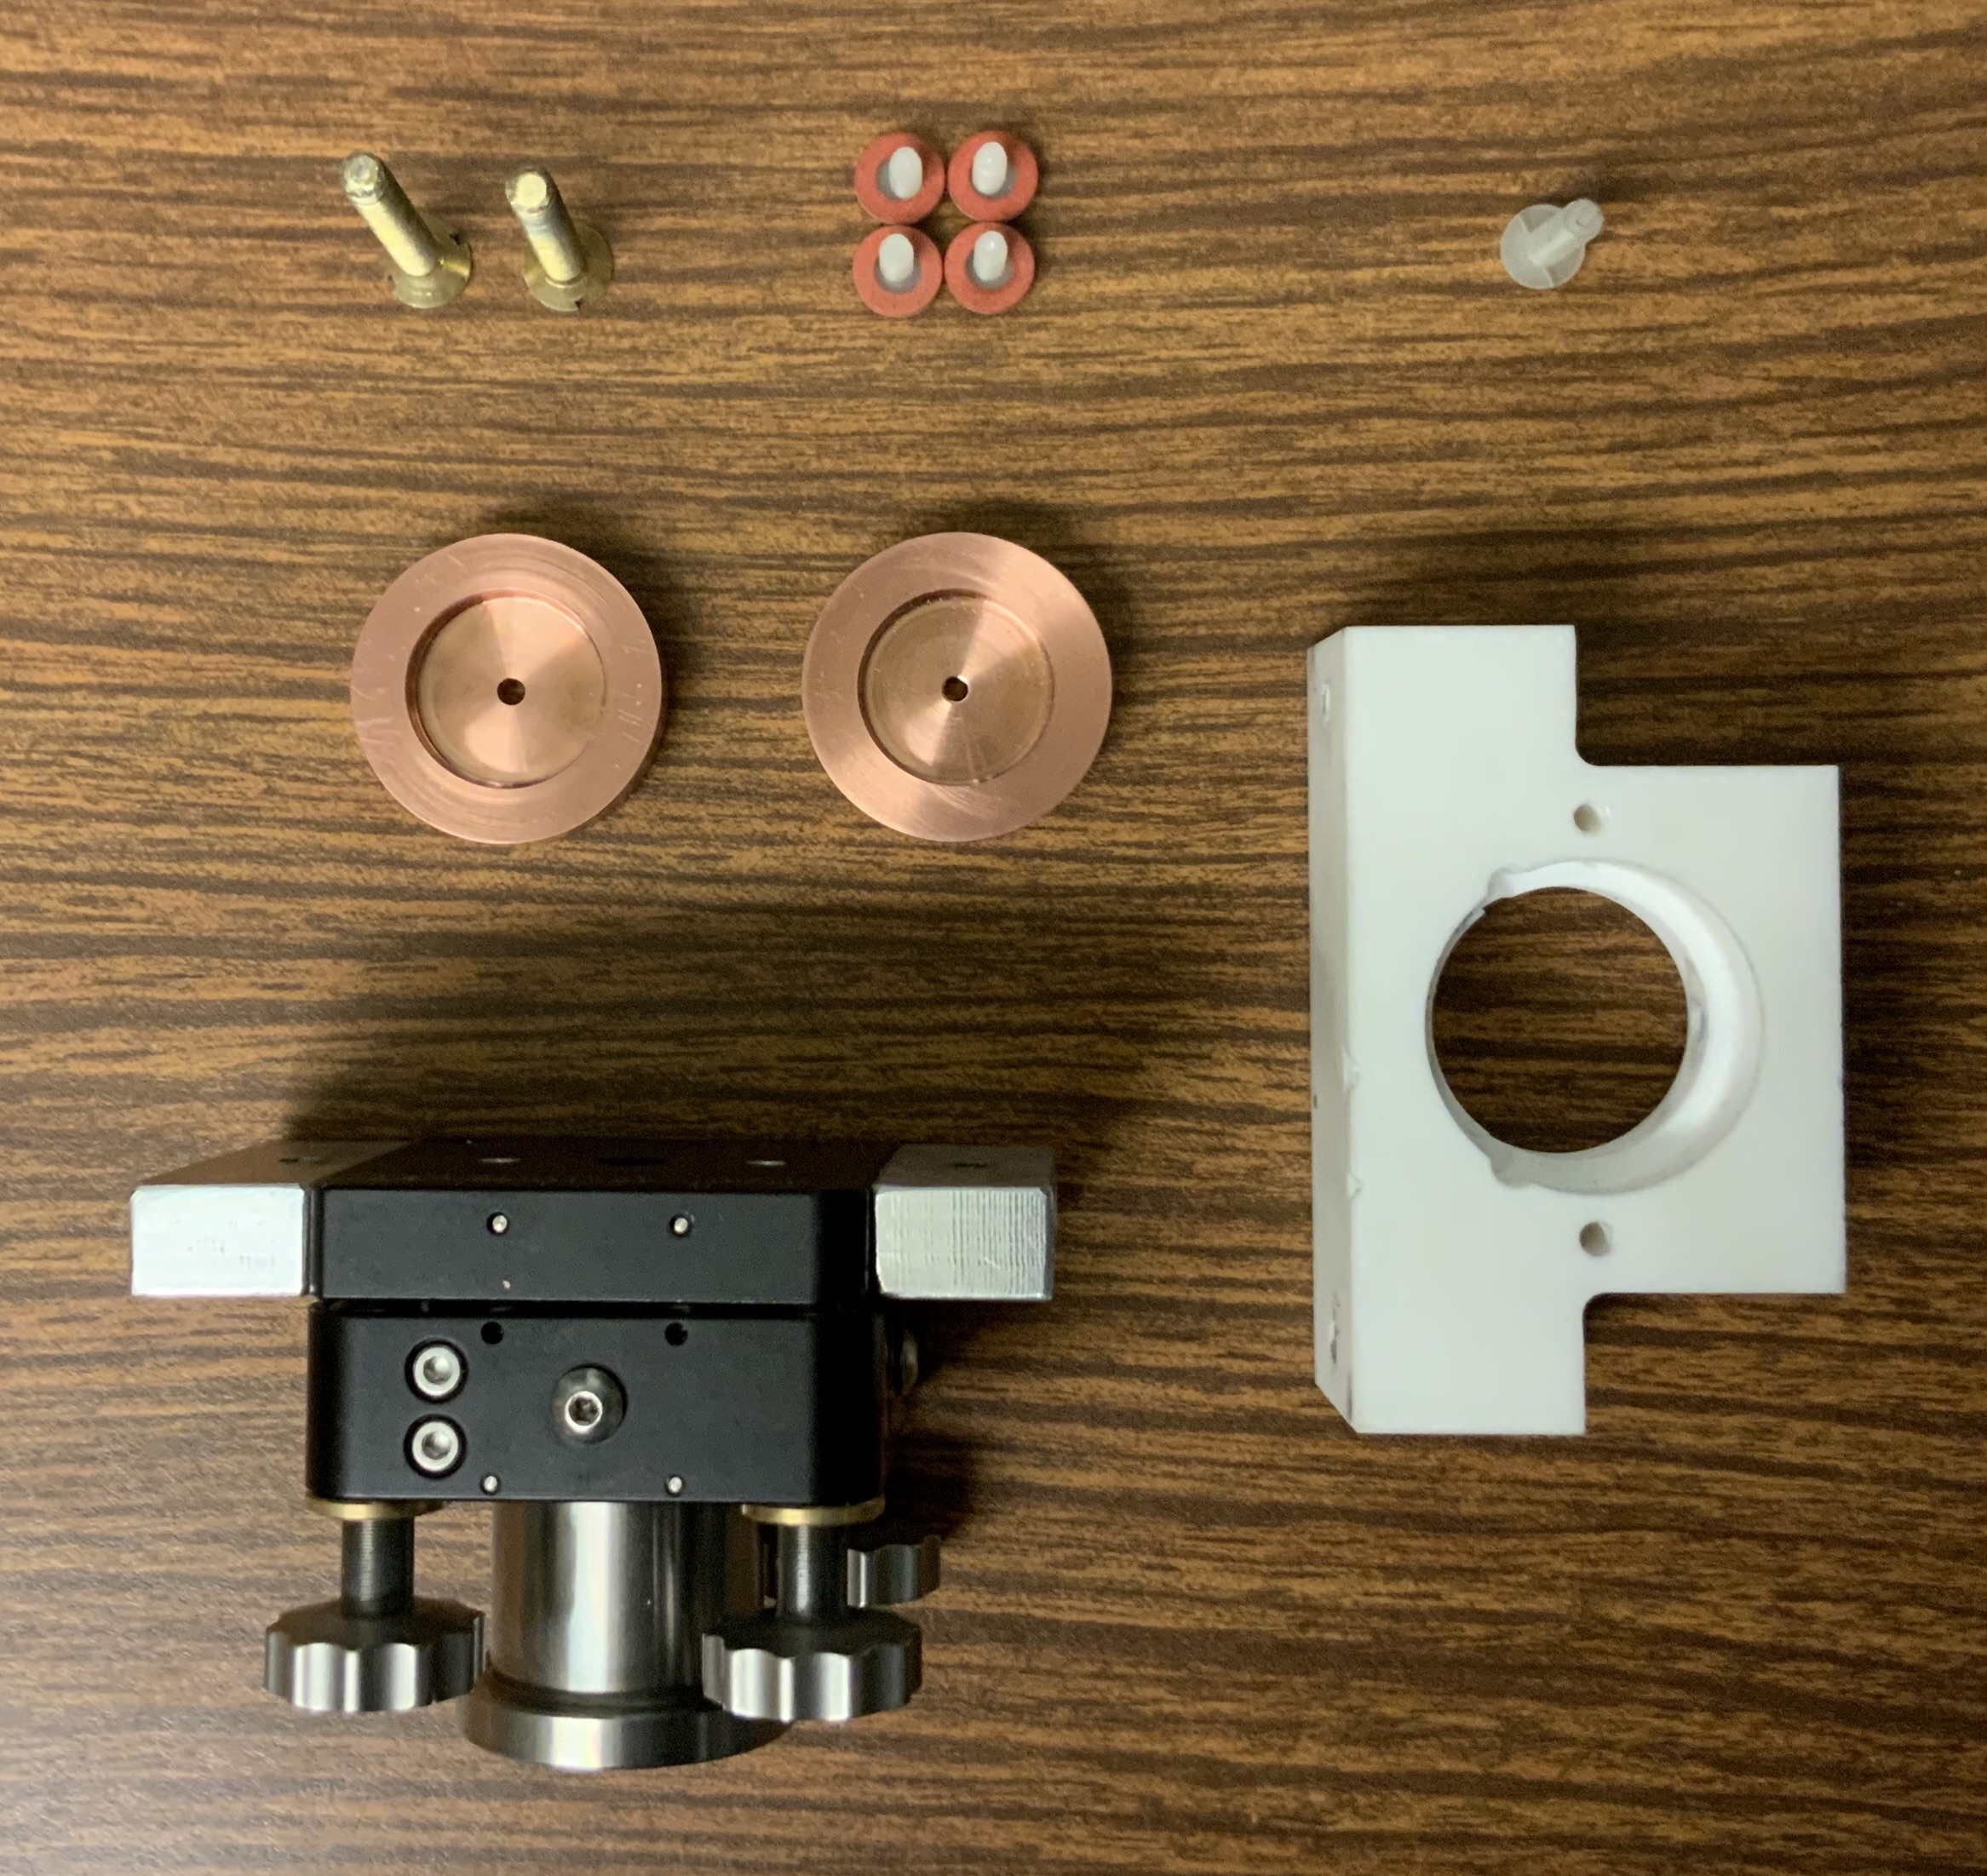
\includegraphics[width=.75\textwidth]{figs/ALGAAS/macor_assembly.jpeg}
\caption{Placeholder for more updated MACOR assembly}
\label{fig:Ez}
\end{figure}
There are two relevant configurations of this experiment: 1) an all-in-one MACOR assembly where the electrodes are mechanically coupled to the optical mount, and 2) larger mechanically decoupled electrode plates.
\\
\\
\textcolor{red}{A lot of time was dedicated towards preliminary mounts made of PLA and PETG. Do I want to do updated measurements and make statements about noise produced from these mounts?}
\\
\\

\subsection{$|E_z|$ strength estimate}
To convey the problem at hand, it is useful to review the illustration seen \textcolor{red}{here (figure showing the the electrode plates, and sample with AlGaAs coating}
\subsubsection{Math}
To find the Electric field screened by the coating we begin with Gauss' Law:

\begin{equation}
\nabla \cdot D = \rho_\mathrm{free}
\end{equation}

For our problem we assume no free charge, but the fused silica substrate with the AlGaAs coating presents dielectric material between the plates. Our initial boundary conditions are also expressed in terms of plate potentials so it is natural to first solve for the potential for every point within our system. We can exploit the cylindrical symmetry with the optic and plate geometry in the $\phi$ coordinate so we shall express the Laplacian accordingly:
\begin{equation}
(1-\chi)\bigg[\frac{1}{\rho}\frac{\partial}{\partial \rho} \bigg( \rho \frac{\partial}{\partial \rho}\bigg) + \frac{\partial^2}{\partial z^2}\bigg]V = 0
\end{equation}

\satoshi{Definition of $\rho$ must be explained. $\rho$ and $\rho_{\mathrm{free}}$ are confusing.
Define $\chi$ and $V$.}
Utilizing this, we can proceed to a construction of a numerical Laplacian.

\subsubsection{Numerical approximation}


\begin{itemize}
\item Potential map computation in cylindrical
\item Computing $E_z$ from potential map
\begin{itemize}
\item inside coating
\item outside coating
\end{itemize}
\end{itemize}


\begin{figure}[H]
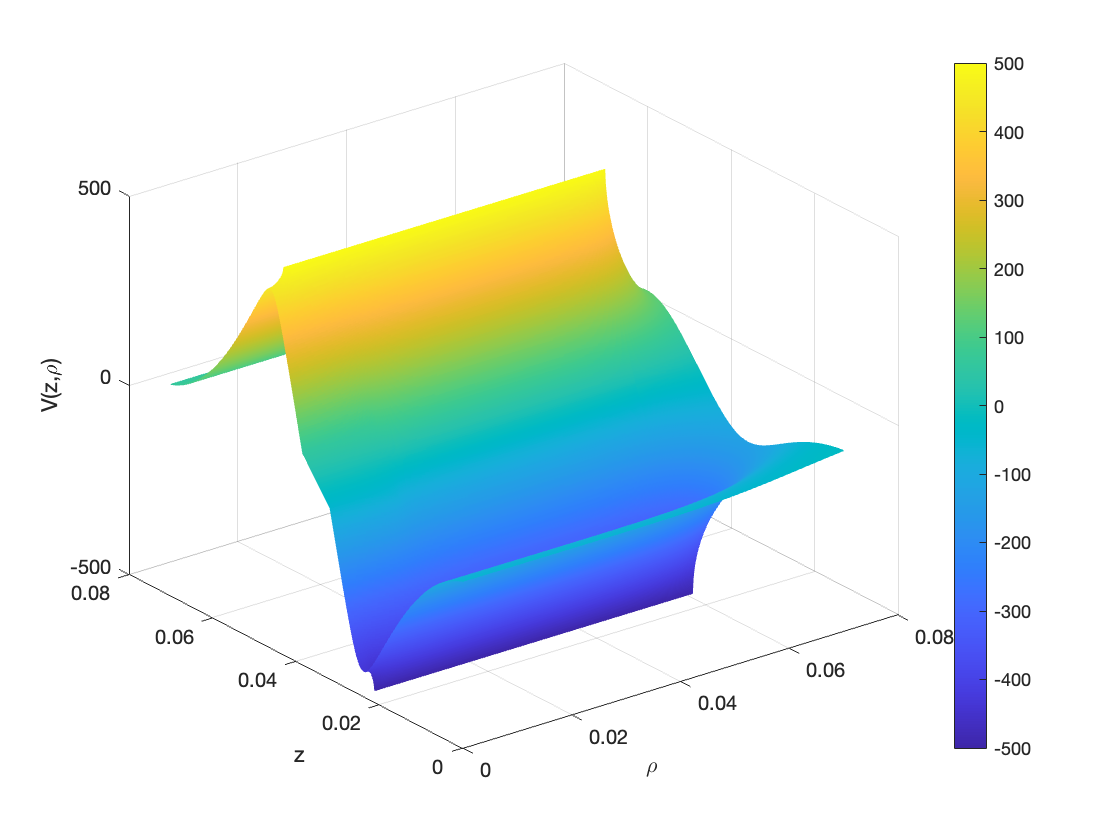
\includegraphics[width=\textwidth]{ALGAAS/13-Sep-2021_potential_map}
\caption{Poisson calculator output potential map ($V(z,\rho)$ in cylindrical coordinates)}
\label{fig:poisson_calc_output}
\end{figure}

\begin{figure}[H]
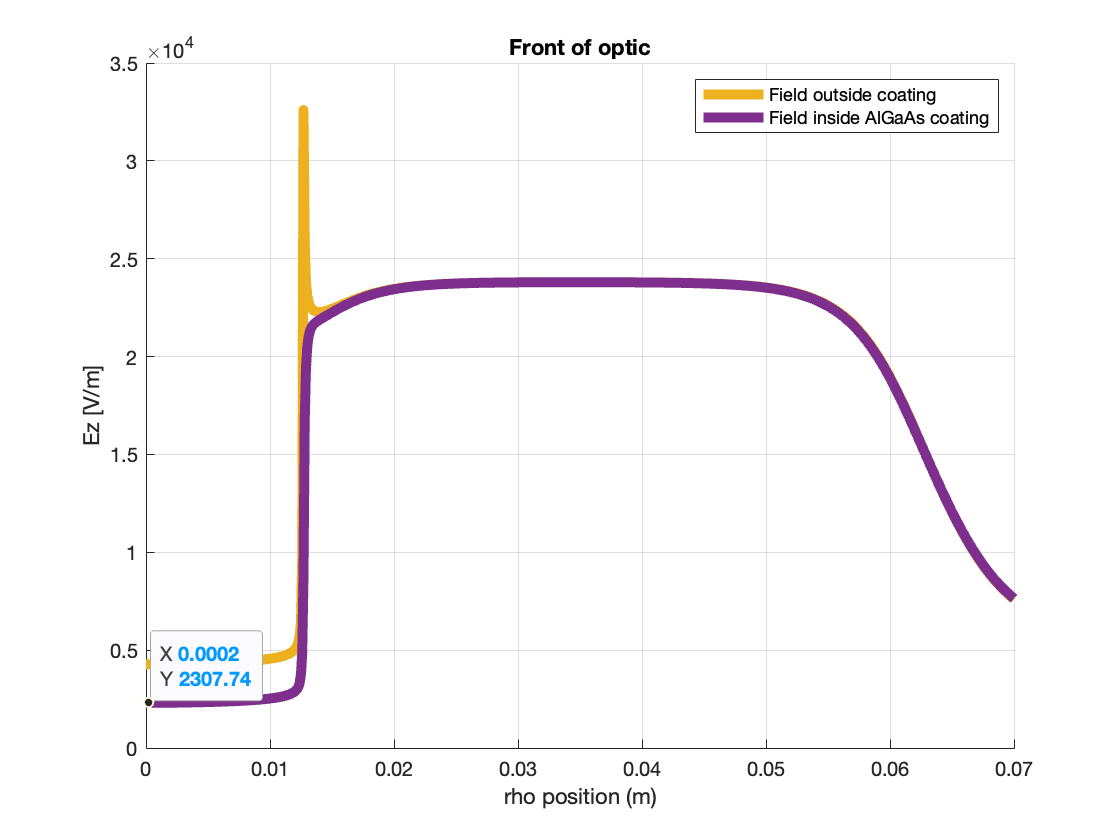
\includegraphics[width=\textwidth]{ALGAAS/13-Sep-2021_e_field_inside_outside_normal}
\caption{$|E_z|$ screened by the scoating and immediately outside AlGaAs coating. \textcolor{red}{Needs to be updated with more current settings}}

\satoshi{How large applied voltage is assumed?}

\label{fig:Ez}
\end{figure}

\begin{figure}[H]
\centering
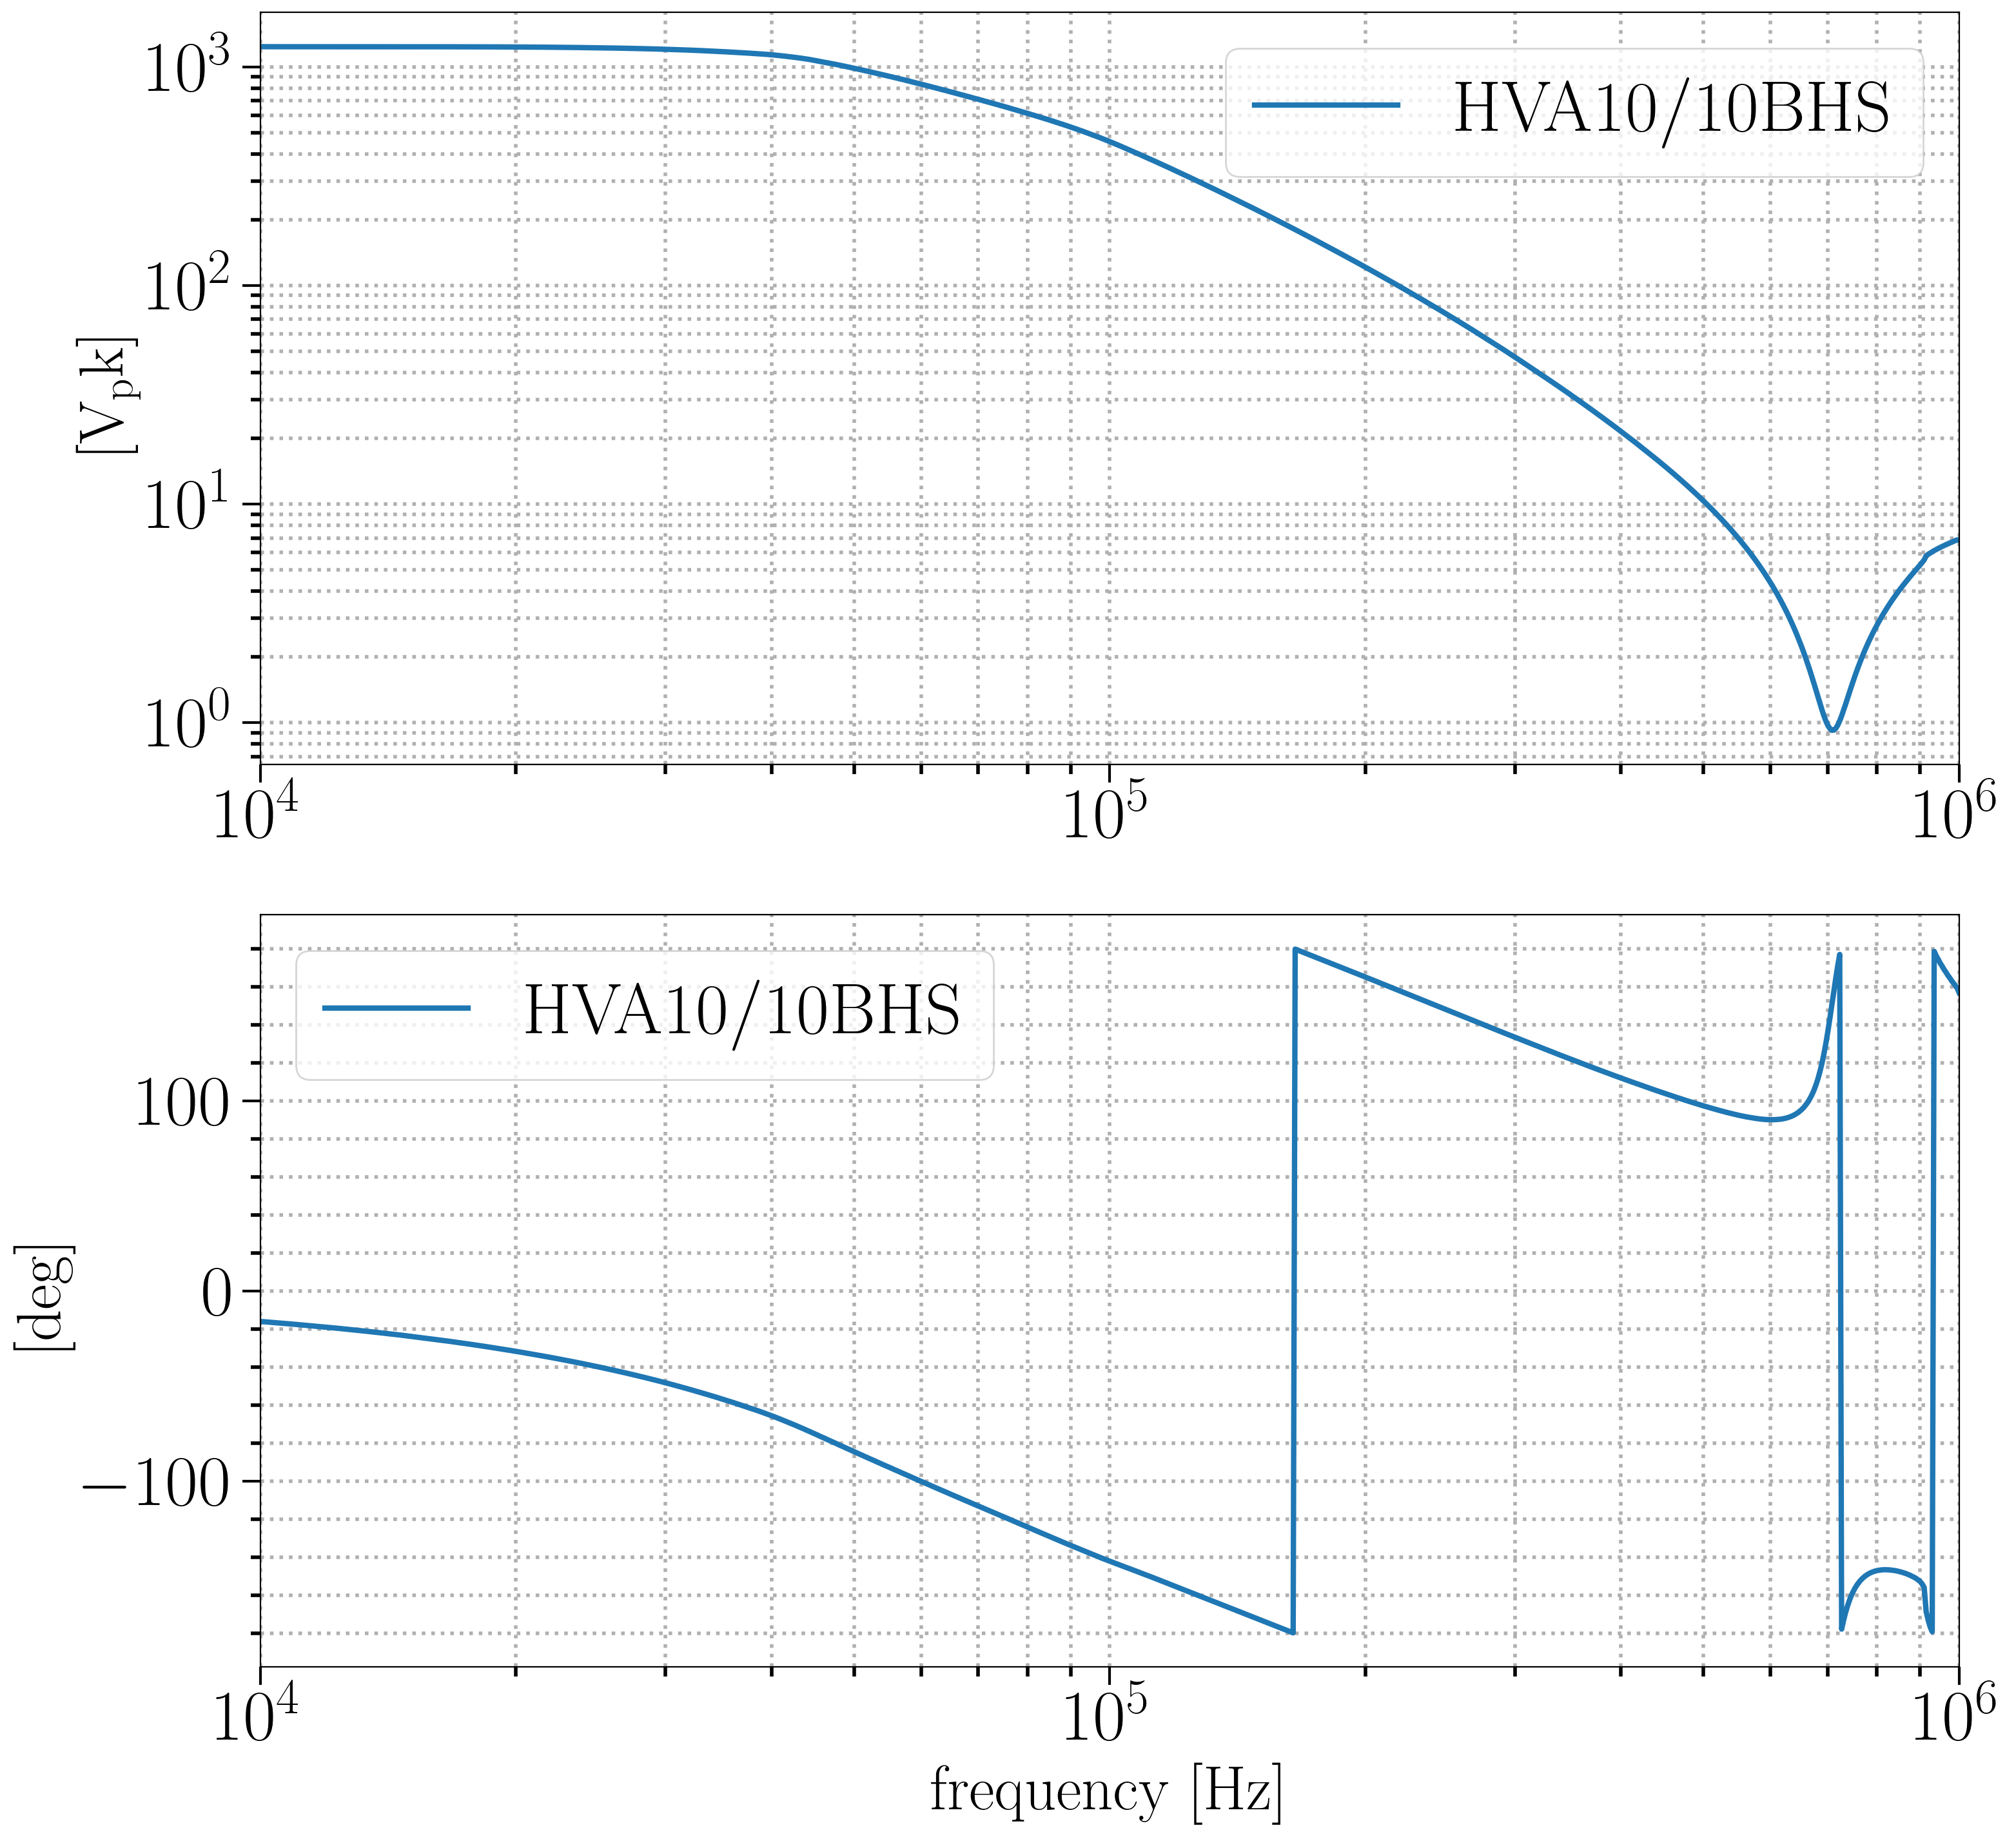
\includegraphics[width=.75\textwidth]{figs/ALGAAS/HVA_TREK1010BHS_1260V_out.png}
\caption{TREK 10/10B-HS HVA frequency dependent measurement. Using Poisson calculator to estimate field strength within coating. (\textcolor{red}{Just HVA for now but will update.} \textcolor{red}{Also, assumes a flat response from coating within this studied region (is this a good assumption or could I do better? (dielectric frequency dependence))}}
\label{fig:Ez}
\end{figure}

\subsection{Calibration}
As discussed, we know that the error signal spectra provides us a voltage spectra that with the above information about the Plant/servo electronics, allows us to
$\mathrm{VFSSOUT}_\mathrm{rms}/\sqrt{Hz} \rightarrow m_\mathrm{rms}/\sqrt{\mathrm{Hz}}$

$$\Delta \mathrm{L} = \mathrm{source}*\alpha(f) \mathrm{A}(f)*\frac{1+\mathrm{OLG}(f)}{\mathrm{OLG}(f)}*\frac{\mathrm{L_{cav}}}{f_\mathrm{laser}}$$

\subsection{Noise Floor}
\subsubsection{Various noise contributions that add up to measured noise floor}
\subsubsection{Shot noise}
Look at the derived shot noise estimate in the appendix V in the Black paper \cite{black_pdh}

\subsubsection{Laser frequency noise}

\begin{itemize}
\item Measure with initial LIGO PMC?
\item There is also a spectra in the Mephisto laser spec sheets
\end{itemize}

\subsubsection{Residual gas noise}


\subsubsection{Mount noise (3D printed mount mechanical noise)}

\subsection{Drive coupling}

\begin{figure}[H]
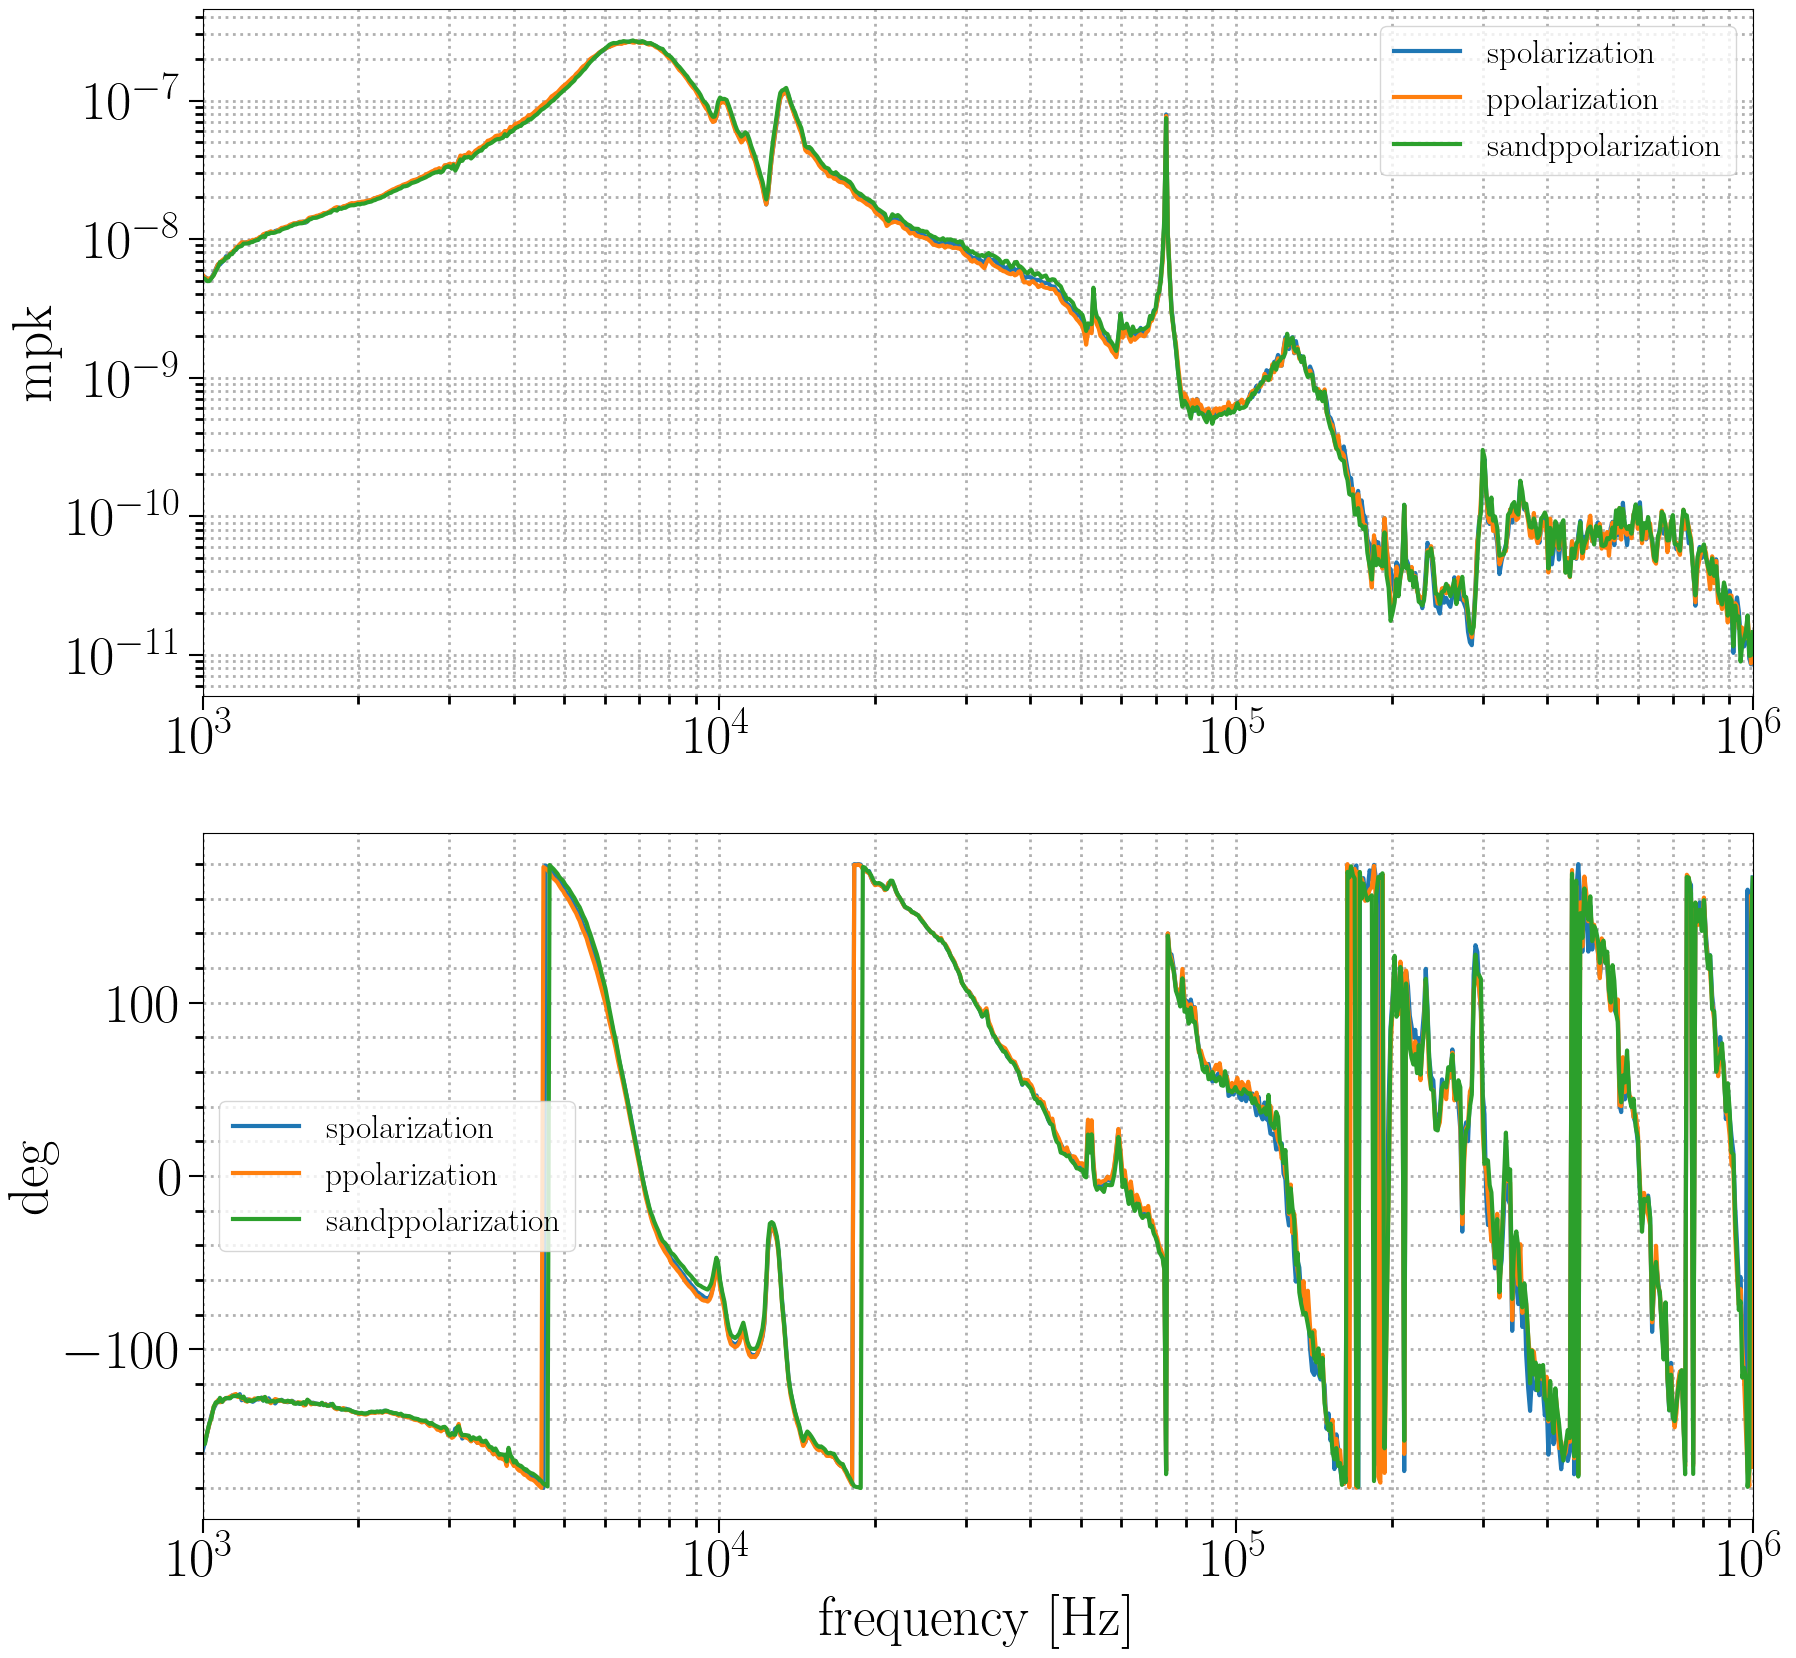
\includegraphics[width=\textwidth]{figs/ALGAAS/cav_polarization_test.png}
\caption{Figure that will include the displacement noise floor, (pockels estimate)*(poisson calculator estimate)*(HVA drive frequency dependence), and the drive coupled measurement \textcolor{red}{figure size needs to be increased}}
\label{fig:measurement_sum}
\end{figure}

\subsubsection{Opto-mechanical coupling}
Sample and mount mechanical mode excitations. Seen with both AlGaAs and a HR coating from an AtFilm (IBS coating)
\begin{itemize}
\item \textbf{Vibration of plates (Leissa)} \cite{leissa} Computing frequencies and order of magnitude
\item \textbf{Steve's COMSOL model results}
\end{itemize}

\subsubsection{Proposed alternative measurement schema}
